\documentclass[12pt,a4paper]{article}
\usepackage[utf8]{inputenc}
\usepackage{amsmath}
\usepackage{amsfonts}
\usepackage{amssymb}
\usepackage{graphicx} % for figure
\usepackage[font=footnotesize]{caption}
\usepackage{subcaption}  % for subfigure
\usepackage{float}
\usepackage{indentfirst} % indent first line after section title
\usepackage{placeins} %FloatBarrier
\usepackage{afterpage}
\usepackage{numprint} % round numbers
\usepackage{siunitx} % round numbers
\usepackage{booktabs}  % nice looking tables

\author{Joao Guilherme Caldas Steinstraesser \\ José Galaz}
\title{Inriamericwaves \\ Report of activities - March-May/16}

\bibliographystyle{abbrv}

\captionsetup[subfigure]{labelformat=parens,labelsep=space}

%% Commands
\newcommand{\der}[1]{\partial_{#1}}
\renewcommand{\epsilon}{\varepsilon}

\renewcommand{\th}{\tilde{h}}
\newcommand{\tu}{\tilde{u}}

\newcommand{\lh}{\overline{h}}
\newcommand{\lu}{\overline{u}}

\newcommand{\opT}{\mathcal{T}}
\newcommand{\opQ}{\mathcal{Q}}
\newcommand{\opIT}{I + \opT}
\newcommand{\opIhT}{I + h\opT\frac{1}{h}}

\newcommand{\Atwo}[2]{\left( \begin{array}{c} #1 \\ #2  \end{array} \right)}

\newcommand{\laplinv}{\mathcal{L}^{-1}}

\begin{document}
\maketitle

\newpage
\tableofcontents

\section{Domain decomposition method for the Serre equations}

\indent Considering that the study and derivation of transparent boundary conditions is much more developed and known for linear partial differential equations \cite{Szeftel2006}, we will consider in the section linearized versions of the Serre equations. The linearization will be performed around constant average water height and velocity, denoted respectively by $h_0$ and $u_0$. Thus, the Serre equations can be written as

\begin{equation}
\label{eq:linearizedSerre}
\begin{cases}
h_t + u_0h_x + h_0u_x = 0 \\
u_t + u_0u_x + gh_x - \frac{h_0^2}{3}(u_{xxt}+u_0u_{xxx}) = 0
\end{cases}
\end{equation} 


\subsection{Linearization with $u_0 = 0$ (for the complete equation)}

\indent Firstly, we will consider the case $u_0 = 0$, which gives, from \eqref{eq:linearizedSerre},

\begin{equation}
\label{eq:linearizedSerre2}
\begin{cases}
h_t + h_0u_x = 0 \\
u_t +  gh_x - \frac{h_0^2}{3}u_{xxt} = 0
\end{cases}
\end{equation} 

\subsubsection{Derivation of the IBCs following \cite{Gander2001B} (rate of convergence of the ASM)}

\indent The derivation of the IBCs will be made analogously as in \cite{Gander2001B}. We will consider the domain $\Omega = \mathcal{R}$ divided in two (possibly overlapped) subdomains, 

\begin{equation*}
\Omega_1 = ]-\infty,L], \qquad \Omega_2 = [0,\infty[
\end{equation*}

\noindent so $L$ denotes the size of the overlap.

\indent We will consider that only one interface boundary condition is imposed, denoted by the operator 

\begin{equation}
	\mathcal{B}_i U(t,x) = \alpha U_x(t,x) + \Lambda_i(U(t,x)) 
\end{equation}

\indent where $U=(h,u)^T$, $i$ indicates the subdomain and $\Lambda_i$ is an linear operator of symbol $\psi_i(s)$ in the Laplace domain.

\indent Thus, the additive Schwarz method is written as

 \begin{equation}
 \label{eq:DDMSerre1}
 \begin{cases}
 h_t^{1,n+1} + h_0 u_x^{1,n+1} = 0, \ t \geq 0, \ x \in \Omega_1 \\
 u_t^{1,n+1} + gh_x^{1,n+1} - \frac{h_0^2}{3}u_{xxt}^{1,n+1} = 0, \ t \geq 0, \ x \in \Omega_1 \\
 \alpha U_x^{1,n+1}(t,L) + \Lambda_1(U_1^{n+1}(t,L)) =   \alpha U_2^{n}(t,L) + \Lambda_1(U_2^{n}(t,L)), \ t\geq 0
 \end{cases}
 \end{equation}
 
  \begin{equation}
   \label{eq:DDMSerre2}
 \begin{cases}
 h_t^{2,n+1} + h_0 u_x^{2,n+1} = 0, \ t \geq 0, \ x \in \Omega_2 \\
 u_t^{2,n+1} + gh_x^{2,n+1} - \frac{h_0^2}{3}u_{xxt}^{2,n+1} = 0, \ t \geq 0, \ x \in \Omega_2 \\
 \alpha U_x^{2,n+1}(t,0) + \Lambda_2(U_2^{n+1}(t,0)) =   \alpha U_1^{n}(t,0) + \Lambda_2(U_1^{n}(t,0)), \ t\geq 0
 \end{cases}
 \end{equation}
 
 \indent Performing the Laplace transform of \eqref{eq:DDMSerre1} and \eqref{eq:DDMSerre2}, one obtains
 
 \begin{equation}
 \label{eq:DDMSerreLaplace1}
 \begin{cases}
 s\hat{h}^{1,n+1} + h_0\hat{u}_x^{1,n+1} = 0, \ s \in \mathcal{C}, \ s > 0, \ x \in \Omega_1 \\
 s\hat{u}^{1,n+1} + g \hat{h}_x^{1,n+1} - s\frac{h_0^2}{3}\hat{u}^{1,n+1}_{xx} = 0, \ s \in \mathcal{C}, \ s > 0, \ x \in \Omega_1  \\
 \alpha \hat{U}_x^{1,n+1}(s,L) + \psi_1\hat{U}^{1,n+1}(s,L) = \alpha \hat{U}_x^{2,n}(s,L) + \psi_1\hat{U}^{2,n}(s,L), \ s \in \mathcal{C} 
 \end{cases}
 \end{equation}
 
  \begin{equation}
 \label{eq:DDMSerreLaplace2}
 \begin{cases}
 s\hat{h}^{2,n+1} + h_0\hat{u}_x^{2,n+1} = 0, \ s \in \mathcal{C}, \ s > 0, \ x \in \Omega_1 \\
 s\hat{u}^{2,n+1} + g \hat{h}_x^{2,n+1} - s\frac{h_0^2}{3}\hat{u}^{2,n+1}_{xx} = 0, \ s \in \mathcal{C}, \ s > 0, \ x \in \Omega_1  \\
 \alpha \hat{U}_x^{1,n+1}(s,0) + \psi_2\hat{U}^{2,n+1}(s,0) = \alpha \hat{U}_x^{1,n}(s,0) + \psi_2\hat{U}^{1,n}(s,0), \ s \in \mathcal{C}
 \end{cases}
 \end{equation}
 
 \indent The solutions of \eqref{eq:DDMSerreLaplace1} and \eqref{eq:DDMSerreLaplace2} have the form
 
 \begin{equation}
 \label{eq:generalSolution}
 \hat{U}^{i,n+1}(s,x) = \overline{U}^{i,n+1}(s)e^{\lambda x}
 \end{equation}
 
 \indent Replacing in \eqref{eq:DDMSerreLaplace1} and \eqref{eq:DDMSerreLaplace2} gives $M\overline{U}^{i,n+1} = 0$, where
 
 \begin{equation}
 M = \left( \begin{array}{c c}
 						s & \lambda h_0 \\
 						\lambda g & s \left(1- \frac{h_0^2\lambda^2}{3} \right) 
 				\end{array} \right)
 \end{equation}
 
 \indent We have nontrivial solutions $\overline{U}^{i,n+1}$ only if $detM = 0$, i.e,
 
 \begin{equation}
 \label{eq:lambda} 
 	\lambda = \pm \sqrt{\frac{s^2}{h_0\left(g+\frac{s^2h_0}{3}\right)}}
 \end{equation}
 
 \indent Considering that the solutions $\hat{U}^{i,n+1}$ must vanish on $\pm \infty$, we have
 
 \begin{equation}
 \hat{U}^{1,n+1} = \overline{U}^{1,n+1}e^{|\lambda|x} \qquad \hat{U}^{2,n+1} = \overline{U}^{2,n+1}e^{-|\lambda|x}
 \end{equation}
 
 \indent The coefficients $\overline{U}^{i,n+1}$ are determined using the boundary conditions in \eqref{eq:DDMSerreLaplace1} and \eqref{eq:DDMSerreLaplace2}. We firstly solve \eqref{eq:DDMSerreLaplace2}, and we get
 
 \begin{equation*}
 \alpha \hat{U}_x^{2,n+1}(s,0) + \psi_2 \hat{U}^{2,n+1}(s,0) = \overline{U}^{2,n+1}(-\alpha|\lambda| + \psi_2) = \alpha \hat{U}_x^{1,n}(s,0) + \psi_2 \hat{U}^{1,n}(s,0)
 \end{equation*}
 
 \noindent so
 
 \begin{equation}
 \label{eq:sol2}
 	\hat{U}^{2,n+1}(s,x) = \frac{\alpha \hat{U}_x^{1,n}(s,0) + \psi_2 \hat{U}^{1,n}(s,0)}{-\alpha|\lambda| + \psi_2} e^{-|\lambda|x} = \frac{\alpha|\lambda| + \psi_2}{-\alpha|\lambda| + \psi_2} \hat{U}^{1,n}(s,0) e^{-|\lambda|x}
 \end{equation}
 
 \indent Similarly, solving \eqref{eq:DDMSerreLaplace1}, we obtain
 
  \begin{equation}
  \label{eq:sol1}
 	\hat{U}^{1,n+1}(s,x) = \frac{\alpha \hat{U}_x^{2,n}(s,L) + \psi_1 \hat{U}^{2,n}(s,L)}{\alpha|\lambda| + \psi_1} e^{|\lambda|(x-L)} = \frac{-\alpha |\lambda| + \psi_1 }{\alpha|\lambda| + \psi_1}\hat{U}^{2,n}(s,L) e^{|\lambda|(x-L)}
 \end{equation}
 
 \noindent and, using \eqref{eq:sol2} in \eqref{eq:sol1}, we get
 
\begin{equation}
 	\hat{U}^{1,n+1}(s,0) = \frac{-\alpha |\lambda| + \psi_1 }{\alpha|\lambda| + \psi_1} \frac{\alpha|\lambda| + \psi_2}{-\alpha|\lambda| + \psi_2} e^{-2|\lambda|L}\hat{U}^{1,n-1}(s,0) 
 \end{equation}
 
 \indent Similarly, using \eqref{eq:sol1} in \eqref{eq:sol2}, 
 
 \begin{equation}
 	\hat{U}^{2,n+1}(s,L) = \frac{-\alpha |\lambda| + \psi_1 }{\alpha|\lambda| + \psi_1} \frac{\alpha|\lambda| + \psi_2}{-\alpha|\lambda| + \psi_2}  e^{-2|\lambda|L}\hat{U}^{2,n-1}(s,L)
 \end{equation}
 
 \indent We can thus define the rate of convergence of the Schwarz method as
 
 \begin{equation}
 \label{eq:rateCV}
 \rho(s,L) = \frac{-\alpha |\lambda| + \psi_1 }{\alpha|\lambda| + \psi_1} \frac{\alpha|\lambda| + \psi_2}{-\alpha|\lambda| + \psi_2}  e^{-2|\lambda|L}
 \end{equation}
 
 \indent In the case $\alpha = 0,\ \psi_1 = \psi_2 = 1$, we recover the classical ASM (with Dirichlet interface boundary condition), and the rate of convergence is 
 
  \begin{equation}
 \rho(s,L)_{classical} = e^{-2|\lambda|L}
 \end{equation}
 
 \indent We can see that, in this case, the ASM converges only if there is an overlapping $L>0$.
 
 \indent The overlapping is not necessary in the general case \eqref{eq:rateCV}. Indeed, choosing $\psi_1 =\alpha |\lambda|$ and $\psi_2 =- \alpha|\lambda|$, the rate of convergence is $ \rho(s,L) \equiv 0$, and the Schwarz method converges after two iterations \cite{Gander2001b}. In this case, the operators for the TBCs, applied respectively in the right boundary of $\Omega_1$ and in the left boundary of $\Omega_2$, are
 
 \begin{equation*}
 	B_1(U) = U_x + |\lambda|U, \qquad B_2(U) = U_x - |\lambda|U
 \end{equation*}
 
 \subsubsection{Derivation of the IBCs following \cite{besse2015} (via the derivation of TBCs)}
 
 \indent In an alternative way, we will follow the approach proposed by \cite{besse2015} to derive the IBCs for the linearized Serre equation \eqref{eq:linearizedSerre2}, and use them as IBCs for the ASM. Being a simpler approach, we will use it in the derivation of IBCs considering other linearizations of the Serre equations.
 
 \indent If we want to solve the problem \eqref{eq:linearizedSerre2} in the finite domain $[a,b]$, the TBCs are constructed by solving it in the complementary of $\Omega$. Thus, we will solve
 
 \begin{equation}
\label{eq:linearizedSerre2Complementary}
\begin{cases}
h_t + u_0h_x + h_0u_x = 0, \ t>0, x<a \ \text{or} \ x >b \\
u_t +  gh_x - \frac{h_0^2}{3}u_{xxt} = 0, \ t>0, x<a \ \text{or} \ x >b  \\
u \longrightarrow 0, \ x \longrightarrow \pm \infty
\end{cases}
\end{equation} 

\indent The approach follows the same arguments as done above. We solve \eqref{eq:linearizedSerre2Complementary} in the Laplace domain, which gives a solution in the form \eqref{eq:generalSolution}, with the two roots $\lambda_i$ of the respective characteristic polynomial given by \eqref{eq:lambda}. To force the solution to vanish in $\pm \infty$, we have the solutions

\begin{gather*}
\hat{U}(s,x) = \overline{U}_-e^{|\lambda(s)|x}, x < a, \\
\hat{U}(s,x) = \overline{U}_+e^{-|\lambda(s)|x}, x > b
\end{gather*}

\indent Thus, from these two solutions we can obtain the following TBCs for solving \eqref{eq:linearizedSerre2} in $\Omega=[a,b]$ :

\begin{gather*}
\hat{U}_x(s,a) - |\lambda(s)|\hat{U}(s,a) = 0 \\
\hat{U}_x(s,b) + |\lambda(s)|\hat{U}(s,b) = 0
\end{gather*}

\noindent respectively for the left and the right boundary of $\Omega$. Approximating $|\lambda(s)|$ by a constant $c>0$  and using these TBCs as IBCs for the ASM, we obtain the operators

 \begin{equation*}
 	B_1(U) = U_x + |c|U, \qquad B_2(U) = U_x - |c|U
 \end{equation*}

\subsection{Linearization with $u_0 \neq 0$ (for the complete equation)}

\indent Following the approach of \cite{besse2015}, we will derive TBCs for the linearized equation :

\begin{equation}
\label{eq:linearizedSerre3} 
\begin{cases}
h_t + u_0h_x + h_0u_x = 0 \\
u_t +  + u_0u_x + gh_x - \frac{h_0^2}{3}(u_{xxt}+u_0u_{xxx}) = 0
\end{cases}
\end{equation} 

\indent We will solve this equation in the complementary of the domain of interest, $\Omega=[a,b]$ :

\indent In the Laplace space, \eqref{eq:linearizedSerre3} is written as

\begin{equation}
\label{eq:linearizedSerre3Laplace} 
\begin{cases}
s\hat{h} + u_0\hat{h}_x + h_0\hat{u}_x = 0 \\
s\hat{u} +  u_0u_x + g\hat{h}_x - \frac{h_0^2}{3}(s\hat{u}_{xxt}+u_0\hat{u}_{xxx})  = 0
\end{cases}
\end{equation} 

\indent Considering a solution in the form $\hat{U}(s,x) = \overline{U}(s)e^{\lambda(s)x}$, and replacing in \eqref{eq:linearizedSerre3Laplace}, we get the linear system $M\overline{U} = 0$, with

\begin{equation*}
M = \left( \begin{array}{c c}
						s + \lambda u_0 & \lambda h_0 \\
						g\lambda & s + u_0\lambda - \frac{h0^2}{3}(\lambda^2 s + \lambda^3 u_0)
				\end{array}
	\right)
\end{equation*}

\indent We have nontrivial solution if and only if $detM = 0$, i.e.,

\begin{equation}
\label{eq:pol4}
s^2 + 2su_0 \lambda + \left( -gh_0 - \frac{h_0^2 s^2}{3} + u_0^2 \right)\lambda^2 - \frac{2}{3}h_0^2u_0s\lambda^3 - \frac{1}{3}h_0^2u_0^2\lambda^4 = 0 
\end{equation}

\indent The roots of \eqref{eq:pol4} (and even their expansions around $s = 0$) have a quite complicated form, but them can be written in the form

\begin{gather*}
	\label{eq:rootsPol4}
	\lambda_1(s) = -\frac{1}{2}(A_1 + A_2) + s \left(-\frac{1}{2u_0} - A_3 - A_4 \right) + O(s^2)  \\
	\lambda_2(s) = \frac{1}{2}(A_1 - A_2) + s \left(-\frac{1}{2u_0} - A_3 + A_4\right) + O(s^2)  \\
	\lambda_3(s) =  -\frac{1}{2}(A_1 - A_2) + s \left(-\frac{1}{2u_0} + A_3 - A_4 \right) + O(s^2) \\
	\lambda_4(s) =  \frac{1}{2}(A_1 + A_2) + s \left(-\frac{1}{2u_0} + A_3 +A_4 \right) + O(s^2) 
\end{gather*} 

\indent Truncating these expressions to order 0, we can see that two of the roots have negative real part, and the other two have positive real part. Let them be named $\lambda^-_1,\lambda^-_2\lambda^+_1,\lambda^+_2$ respectively.

\indent Moreover, from the polynomial \eqref{eq:pol4}, we get the relations

\begin{gather}
	\label{eq:girardPol4A}
	\lambda^-_1 + \lambda^-_2 + \lambda^+_1 + \lambda^+_2 = \frac{\frac{2}{3} h_0^2u_0s}{-\frac{1}{3} h_0^2u_0^2} = \frac{-2s}{u_0} \\
	\label{eq:girardPol4B}
	\lambda^-_1 \lambda^-_2 \lambda^+_1 \lambda^+_2 = \frac{s^2}{-\frac{1}{3} h_0^2u_0^2} = \frac{-3s^2}{h_0^2u_0^2}
\end{gather}

\indent The solutions of \eqref{eq:linearizedSerre3} in the complementary of $[a,b]$ are

\begin{gather*}
	\hat{U}(s,x) = \overline{U}^+_1e^{\lambda^+_1(s)x} + \overline{U}^+_2e^{\lambda^+_2(s)x}, x < a, \\
	\hat{U}(s,x) = \overline{U}^-_1e^{\lambda^-_1(s)x} + \overline{U}^-_2e^{\lambda^-_2(s)x}, x > b
\end{gather*}

\indent from which we can derive the TBCs

\begin{gather*}
\hat{u}(s,a) - (\lambda^+_1(s) + \lambda^+_2(s))\hat{u}_x(s,a) + \lambda^+_1(s) \lambda^+_2(s)\hat{u}_{xx}(s,a) = 0 \\
\hat{u}(s,b) - (\lambda^-_1(s) + \lambda^-_2(s))\hat{u}_x(s,b) + \lambda^-_1(s) \lambda^-_2(s)\hat{u}_{xx}(s,b) = 0 \\
\end{gather*}

\indent respectively for the left and the right boundaries of $[a,b]$. Using the relations \eqref{eq:girardPol4A}  and \eqref{eq:girardPol4B} We propose to approximate the TBCs using three constants, $c_1,c_2,c_3$, such that : 

\begin{gather*}
	\lambda^-_1 + \lambda^-_2 = c_1 \\
	\lambda^-_1 \lambda^-_2 = c_2  \\
	 \lambda^+_1 + \lambda^+_2 = -2 c_3 - c_1 \\
	 \lambda^+_1 \lambda^+_2 = -\frac{3c_3^2}{c_2h_0}
\end{gather*} 

\noindent giving the IBC operators

\begin{equation}
	B_1(U) = U  - c_1U_x + c_2 U_{xx}, \qquad B_2(U) = U + (2 c_3 + c_1)U_x - \frac{3c_3^2}{c_2h_0} U_{xx}
\end{equation}

\noindent applied respectively in the right and the left boundaries.

\subsection{Linearization with $u_0 \neq 0$ (only for the dispersive equation)}

\indent Considering that we solve the Serre equations with a splitting method, we will derive IBCs for each one of the splitting steps. In the following paragraphs, we will consider the dispersive equation :

\begin{equation}
 \label{eq:dispersiveSerre}
	\begin{cases}
		h_t = 0 \\
		u_t - \frac{1}{3h} \left( h^3 \left( u_{xt} + uu_{xx} - (u_x)^2\right) \right)_x = 0
	\end{cases}
\end{equation}

\indent We can work only with the second equation of \eqref{eq:dispersiveSerre}. Linearizing it around $h0$ and $u_0$, we obtain

\begin{equation}
	\label{eq:linearizedSerre4}
	u_t - \frac{h_0^2}{3}(u_{xxt}+u_0u_{xxx}) = 0
\end{equation}

\indent We will solve this equation in the complementary of $[a,b]$ in order to compute its TBcs. In the Laplace space, \eqref{eq:linearizedSerre4} reads

\begin{equation}
	\label{eq:linearizedSerre4Laplace}
	s \hat{u} - \frac{h_0^2}{3}(s\hat{u}_{xx}+u_0\hat{u}_{xxx}) = 0
\end{equation}

\noindent which admits a solution in the general form $\hat{u}(s,x) = \overline{u}(\lambda)e^{\lambda(s)x}$. Replacing in \eqref{eq:linearizedSerre4Laplace}, we obtain the characteristic polynomial

\begin{equation}
\label{eq:pol3}
3s - h_0^2s\lambda^2 - h0^2u_0\lambda^3 = 0
\end{equation}

\indent The roots of \eqref{eq:pol3} verifies, for $u_0 > 0$ (??????)

\begin{equation*}
	Re(\lambda_1) > 0, \qquad Re(\lambda_2) < 0, \qquad Re(\lambda_3) < 0 
\end{equation*}

\noindent and the relations

\begin{gather}
	\label{eq:girardPol3A}
		\lambda_1 + \lambda_2 + \lambda_3 = \frac{h_0^2s}{- h0^2u_0} = -\frac{s}{u_0} \\
	\label{eq:girardPol3B}
		\lambda_1 \lambda_2 \lambda_3 = \frac{3s}{h0^2u_0}
\end{gather}

\noindent so the solution of \eqref{eq:linearizedSerre4Laplace} has the form

\begin{gather*}
	\hat{u}(s,x) = \overline{u}_1(s)e^{\lambda_1(s)x}, x < a, \\
	\hat{u}(s,x) = \overline{u}_2(s)e^{\lambda_2(s)x} + \overline{u}_3(s)e^{\lambda_3(s)x}, x > b
\end{gather*}

\noindent from which we can derive the TBCs

\begin{gather*}
\frac{1}{\lambda_1(s)}\hat{u}_{x}(s,a) - u(s,a) = 0 \qquad \frac{1}{\lambda_1^2(s)}\hat{u}_{xx}(s,a) - u(s,a) = 0 \\
\hat{u}(s,b) - (\lambda_2(s) + \lambda_3(s))\hat{u}_x(s,b) + \lambda_2(s) \lambda_3(s)\hat{u}_{xx}(s,b) = 0 \\
\end{gather*}

\indent Taking into account the relations \eqref{eq:girardPol3A} and \eqref{eq:girardPol3B}, we propose to approximate the TBCs using two constants, $c_1$ and $c_2$, such that

\begin{gather*}
	\lambda_1 = c_1 \\
	\lambda_2 + \lambda_3 = - c_2 - c_1 \\
	\lambda_2 \lambda_3 = \frac{3c_2}{h_0^2c_1}
\end{gather*}

\noindent giving the IBC operators

\begin{equation}
	B_1(u) = u - \frac{1}{c_1}u_{x}, \qquad B_2(u) = u - \frac{1}{c_1^2}u_{xx}, \qquad B_3(u) = u + (c_2+c_1)u_x + \frac{3c_2}{h_0^2c_1} u_{xx}
\end{equation}

\indent In the DDM, $B_1$ and $B_2$ should be applied as IBC in the left boundary of right domain, and $B_3$ as IBC in the right boundary of left domain.


\subsubsection{Tests with the approximate TBCs}

\indent In order to study this proposed approximations and find the coefficients that provide the best TBCs (and possibly some dependence on the linearization parameter $u_0$), we solved the linearized equation \eqref{eq:linearizedSerre4}, with $0 \leq t \leq 10$ for different pairs $(c_1,c_2) \in [-10,10]^2$ and computed for each case the error

\begin{equation*}
e(c_1,c_2) = ||u^{c1,c2}-u^{ref}|| = \sqrt{\Delta t \Delta x \sum_{n=0}^T {\sum_{i=0}^N{(u_i^{n,c_1,c_2} - u_i^{n,ref})^2} }}
\end{equation*}

\indent Two problems were solved, the first one with a wave moving to the right, and the second one with a wave moving to both directions. The initial solution $u_0$ in both cases is the solitary cnoidal solution, and the movement is forced by the respective $h$ solution of the Serre equations ($h$ is not modified in the dispersive part of the system).

\indent For both tests, we obtained the following conclusions:

\begin{itemize}
\item For $c_2 \neq 0$, the error  $e(c_1,c_2)$ is independent of $c_2$.
\item $c_2 = 0$ provides much better results than $c_2 = 0$, especially in the first problem.
\item The best results are provided by $c_1 \in [-1,1]$ 
\end{itemize}

\indent With $c_2 = 0$, the TBCs are written as

\begin{gather*}
\frac{1}{c_1}u_{x}(t,a) -  u(t,a) = 0 \qquad \frac{1}{c_1^2}u _{xx}(t,a) - u(t,a) = 0 \\
u(t,b) + c_1 u_x(t,b)  = 0 \\
\end{gather*}

\section{Appendix : study of sign of roots in the case of linearization with $u_0 \neq 0$ (only for the dispersive equation)}

\indent The roots of \eqref{eq:pol3} are

\begingroup
\scriptsize
\begin{equation}
	\label{eq:lambdaExacts}
	\begin{aligned}
	&& \lambda_1\left( {{h_0}}, {{u_0}}, s \right) = & \frac{2^{\frac{1}{3}} \left(-\frac{{{h_0}}^{2} {{u_0}}^{3}}{2 \, {{h_0}}^{2} s^{3} - 81 \, s {{u_0}}^{2} - 9 \, \sqrt{-4 \, {{h_0}}^{2} s^{2} + 81 \, {{u_0}}^{2}} s {{u_0}}}\right)^{\frac{1}{3}} s^{2}}{3 \, {{u_0}}^{2}} + \\
	&& & {\left(\frac{\sqrt{-4 \, {{h_0}}^{2} s^{2} + 81 \, {{u_0}}^{2}} s}{6 \, {{h_0}}^{2} {{u_0}}^{2}} - \frac{2 \, {{h_0}}^{2} s^{3} - 81 \, s {{u_0}}^{2}}{54 \, {{h_0}}^{2} {{u_0}}^{3}}\right)}^{\frac{1}{3}} - \frac{s}{3 \, {{u_0}}} \\
	&& \lambda_2\left( {{h_0}}, {{u_0}}, s \right) = & -\frac{1}{12} \cdot 2^{\frac{2}{3}} {\left(i \, \sqrt{3} + 1\right)} \left(-\frac{2 \, {{h_0}}^{2} s^{3} - 81 \, s {{u_0}}^{2} - 9 \, \sqrt{-4 \, {{h_0}}^{2} s^{2} + 81 \, {{u_0}}^{2}} s {{u_0}}}{{{h_0}}^{2} {{u_0}}^{3}}\right)^{\frac{1}{3}}\\
	&& & + \frac{2^{\frac{1}{3}} \left(-\frac{{{h_0}}^{2} {{u_0}}^{3}}{2 \, {{h_0}}^{2} s^{3} - 81 \, s {{u_0}}^{2} - 9 \, \sqrt{-4 \, {{h_0}}^{2} s^{2} + 81 \, {{u_0}}^{2}} s {{u_0}}}\right)^{\frac{1}{3}} s^{2} {\left(i \, \sqrt{3} - 1\right)}}{6 \, {{u_0}}^{2}} - \frac{s}{3 \, {{u_0}}} \\
	&& \lambda_3\left( {{h_0}}, {{u_0}}, s \right) = & \frac{1}{12} \cdot 2^{\frac{2}{3}} {\left(i \, \sqrt{3} - 1\right)} \left(-\frac{2 \, {{h_0}}^{2} s^{3} - 81 \, s {{u_0}}^{2} - 9 \, \sqrt{-4 \, {{h_0}}^{2} s^{2} + 81 \, {{u_0}}^{2}} s {{u_0}}}{{{h_0}}^{2} {{u_0}}^{3}}\right)^{\frac{1}{3}} +\\
	&& & \frac{2^{\frac{1}{3}} \left(-\frac{{{h_0}}^{2} {{u_0}}^{3}}{2 \, {{h_0}}^{2} s^{3} - 81 \, s {{u_0}}^{2} - 9 \, \sqrt{-4 \, {{h_0}}^{2} s^{2} + 81 \, {{u_0}}^{2}} s {{u_0}}}\right)^{\frac{1}{3}} s^{2} {\left(-i \, \sqrt{3} - 1\right)}}{6 \, {{u_0}}^{2}} - \frac{s}{3 \, {{u_0}}}
	\end{aligned}
\end{equation}
\endgroup

\indent A Taylor expansion of these roots around $s = 0$ give

\begin{equation}
	\label{eq:taylor3}
	\begin{aligned}
		&& \lambda_1\left( {{h_0}}, {{u_0}}, s \right) = & \frac{3^{\frac{1}{3}} s^{\frac{1}{3}}}{{{h_0}}^{\frac{2}{3}} {{u_0}}^{\frac{1}{3}}} + \mathcal{O}(s) \\
		&& \lambda_2\left( {{h_0}}, {{u_0}}, s \right) = & \frac{2^{\frac{2}{3}} {\left(-i \cdot 6^{\frac{1}{3}} \sqrt{3} {{h_0}}^{\frac{1}{3}} {{u_0}}^{\frac{2}{3}} - 6^{\frac{1}{3}} {{h_0}}^{\frac{1}{3}} {{u_0}}^{\frac{2}{3}}\right)} s^{\frac{1}{3}}}{4 \, {{h_0}} {{u_0}}} + \mathcal{O}(s) = \\
		&& = & -C sign(u) s^{\frac{1}{3}} \left( \frac{1}{2} + i\frac{\sqrt{3}}{2}\right) + \mathcal{O}(s) = \\
		&& = & -C sign(u) s^{\frac{1}{3}} e^{i\frac{\pi}{3}} + \mathcal{O}(s) \\
		&& \lambda_3\left( {{h_0}}, {{u_0}}, s \right) = & \frac{2^{\frac{2}{3}} {\left(i \cdot 6^{\frac{1}{3}} \sqrt{3} {{h_0}}^{\frac{1}{3}} {{u_0}}^{\frac{2}{3}} - 6^{\frac{1}{3}} {{h_0}}^{\frac{1}{3}} {{u_0}}^{\frac{2}{3}}\right)} s^{\frac{1}{3}}}{4 \, {{h_0}} {{u_0}}} + \mathcal{O}(s) = \\
		&& = & C sign(u) s^{\frac{1}{3}} \left( -\frac{1}{2} + i\frac{\sqrt{3}}{2}\right) + \mathcal{O}(s) = \\
		&& = & C sign(u) s^{\frac{1}{3}} e^{i\frac{2\pi}{3}} + \mathcal{O}(s) \\
	\end{aligned}
\end{equation}

\noindent where

\begin{equation*}
	C = \frac{\left(24h_0u_0^2\right)^{\frac{1}{3}}}{2h_0|u_0|} > 0
\end{equation*}

\indent The Laplace frequencies $s$ are supposed to have positive real part. Writing $s = \rho e ^{i\theta}$, that implies

\begin{equation*}
	\theta \in \left] -\frac{\pi}{2}, \frac{\pi}{2} \right[
\end{equation*}

\indent and therefore

\begin{equation}
\label{eq:domaineAngles}
\begin{gathered}
	\frac{\theta}{3} \in \left] -\frac{\pi}{6}, \frac{\pi}{6} \right[ \\
	\frac{\theta}{3} + \frac{\pi}{3} \in \left] \frac{\pi}{6}, \frac{\pi}{2} \right[ \\
	\frac{\theta}{3} + \frac{2\pi}{3} \in \left] \frac{\pi}{2}, \frac{5\pi}{6} \right[
\end{gathered}
\end{equation}

\indent Truncating the Taylor expansions \eqref{eq:taylor3} at the first term and using the trigonometric form of $s$, we have

\begin{equation}
	\label{eq:seriesTrunc}
	\begin{aligned}
	\lambda_1\left( {{h_0}}, {{u_0}}, s \right) = & \frac{3^{\frac{1}{3}} \rho^{\frac{1}{3}}}{{{h_0}}^{\frac{2}{3}} {{u_0}}^{\frac{1}{3}}} e^{i\frac{\theta}{3}} \\
	\lambda_2\left( {{h_0}}, {{u_0}}, s \right) = & -C sign(u) \rho^{\frac{1}{3}} e^{i \left( \frac{\theta}{3}  + \frac{\pi}{3} \right)} \\
	\lambda_3\left( {{h_0}}, {{u_0}}, s \right) = & C sign(u) \rho^{\frac{1}{3}} e^{i \left( \frac{\theta}{3}  + \frac{2\pi}{3} \right)}
	\end{aligned}
\end{equation}

\indent From \eqref{eq:domaineAngles} and \eqref{eq:seriesTrunc}, it is clear that

\begin{equation*}
	sign(Re(\lambda_1)) = sign(u),  \qquad sign(Re(\lambda_2)) = -sign(u), \qquad sign(Re(\lambda_3)) = -sign(u)
\end{equation*}

\indent As an example, the figures \ref{fig:cas1} to \ref{fig:cas3} show the real part of the roots (computed using the exact expressions \eqref{eq:lambdaExacts}) in function of $h_0$ for some fixed values of $s$ and $u_0$ (the values were chosen varying the magnitude and the sign of $Im(s)$ and $u_0$).

\begingroup
	\noindent
	\begin{minipage}{.5\linewidth}
		\centering
		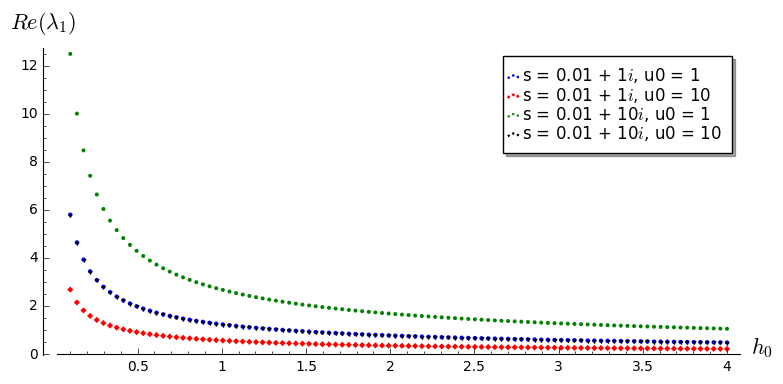
\includegraphics[scale=.35]{{Figures/LinDispersive/l1A}.png}
		\captionof{subfigure}{$Re(\lambda_1)$}
	\end{minipage}
	\begin{minipage}{.5\linewidth}
		\centering
		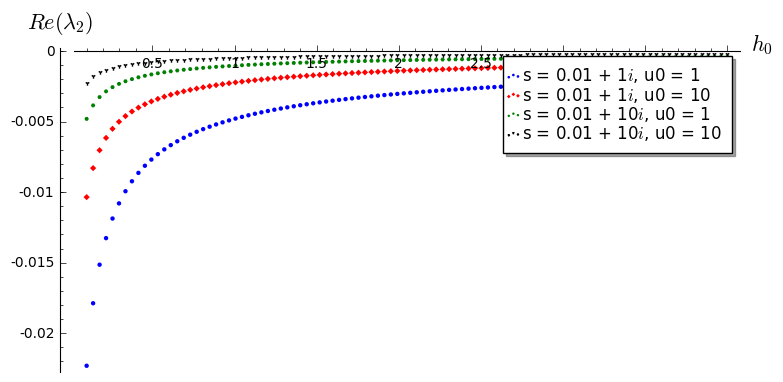
\includegraphics[scale=.35]{{Figures/LinDispersive/l2A}.png}
		\captionof{subfigure}{$Re(\lambda_2)$}
	\end{minipage}
	\begin{minipage}{1.\linewidth}
		\centering
		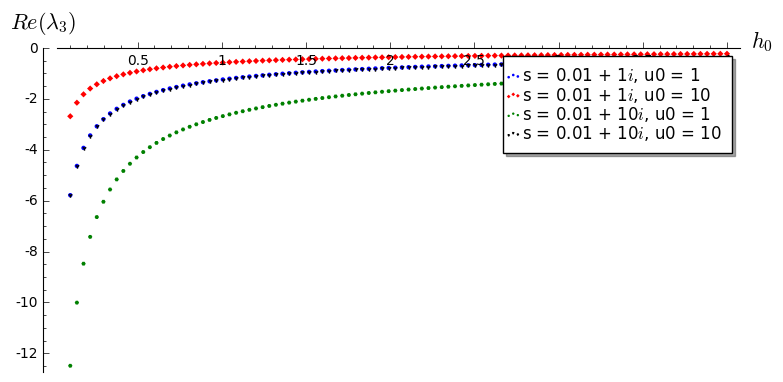
\includegraphics[scale=.35]{{Figures/LinDispersive/l3A}.png}
		\captionof{subfigure}{$Re(\lambda_3)$}
	\end{minipage}
	\captionof{figure}{Cas 1 \label{fig:cas1}}
\endgroup

\begingroup
	\noindent
	\begin{minipage}{.5\linewidth}
		\centering
		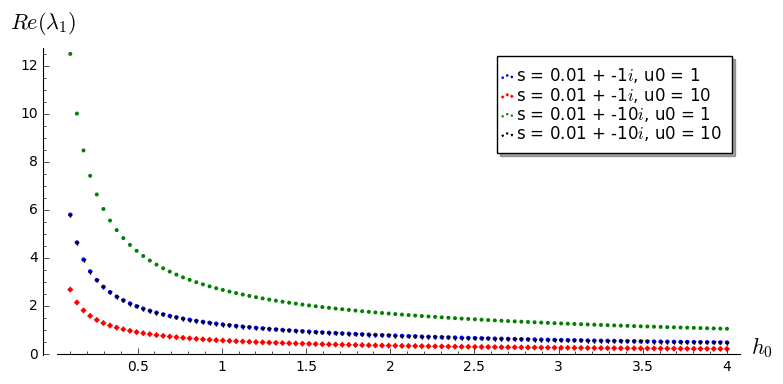
\includegraphics[scale=.35]{{Figures/LinDispersive/l1B}.png}
		\captionof{subfigure}{$Re(\lambda_1)$}
	\end{minipage}
	\begin{minipage}{.5\linewidth}
		\centering
		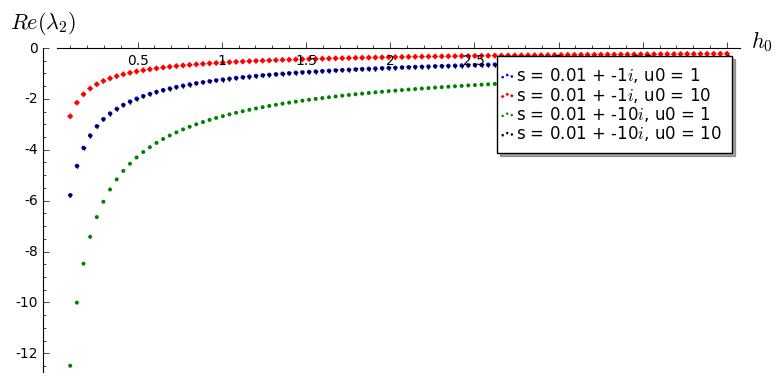
\includegraphics[scale=.35]{{Figures/LinDispersive/l2B}.png}
		\captionof{subfigure}{$Re(\lambda_2)$}
	\end{minipage}
	\begin{minipage}{\linewidth}
		\centering
		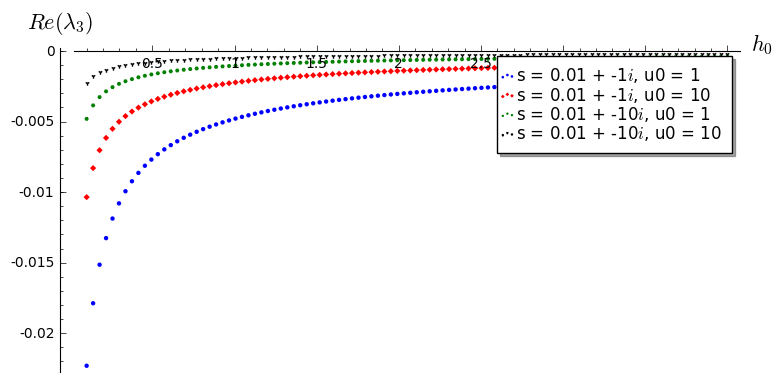
\includegraphics[scale=.35]{{Figures/LinDispersive/l3B}.png}
		\captionof{subfigure}{$Re(\lambda_3)$}
	\end{minipage}
	\captionof{figure}{Cas 2 \label{fig:cas2}}
\endgroup

\begingroup
\noindent
	\begin{minipage}{.5\linewidth}
		\centering
		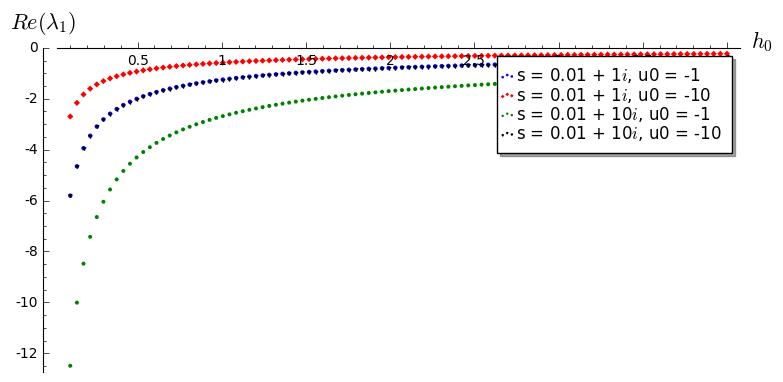
\includegraphics[scale=.35]{{Figures/LinDispersive/l1C}.png}
		\captionof{subfigure}{$Re(\lambda_1)$}
	\end{minipage}
	\begin{minipage}{.5\linewidth}
		\centering
		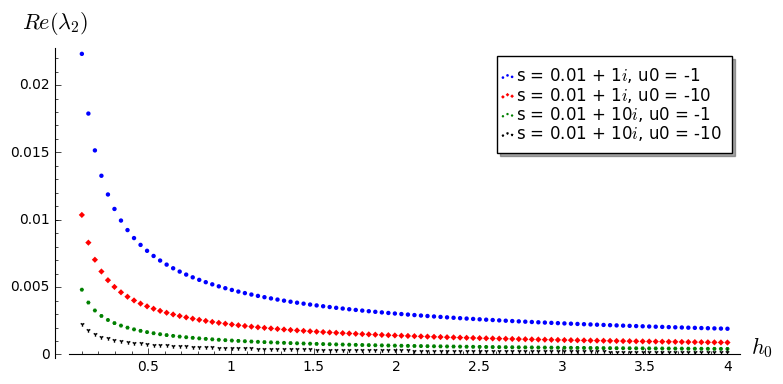
\includegraphics[scale=.35]{{Figures/LinDispersive/l2C}.png}
		\captionof{subfigure}{$Re(\lambda_2)$}
	\end{minipage}
	\begin{minipage}{\linewidth}
		\centering
		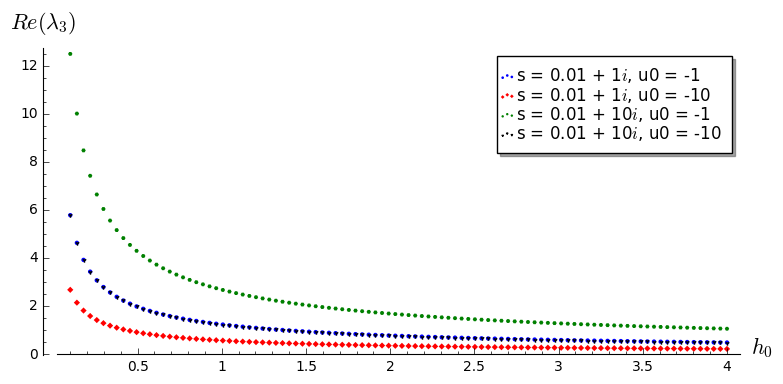
\includegraphics[scale=.35]{{Figures/LinDispersive/l3C}.png}
		\captionof{subfigure}{$Re(\lambda_3)$}
	\end{minipage}
	\captionof{figure}{Cas 3 \label{fig:cas3}}
\endgroup
\newpage
	
\FloatBarrier
\bibliography{../may/biblio}

\end{document}
